\documentclass[11pt]{beamer}
\usepackage{hyperref}
\usepackage[czech]{babel}
\usepackage[utf8]{inputenc}
\usepackage{graphics}
\usepackage{listings}
\usetheme{Darmstadt}
\usecolortheme{wolverine}

\title{Řadící algoritmy - Řazení záměnou}
\author[Václav Doleček]{Václav Doleček\\
{\small \href{xdolec03@stud.fit.vutbr.cz}{\texttt{xdolec03@stud.fit.vutbr.cz}}}}
\institute[VUT]{Vysoké učení technické \\ Fakulta informačných technológií}
\date{\today}

\begin{document}
 
\frame{\titlepage}

 
\begin{frame}[fragile]{Úvod do problematiky Řadících altoritmů}
\begin{itemize}
    \item Řazení/třízení je jedna z~nejzákladnějších operací co musí počítat zvládat. Jedno jestli řadí lidi v~tabulce podle datumu narození, nebo seřazuje a uspořádává místo data na disku, počítače se bez toho neobejdou, neboť neuspořádaná data nejsou jen tak.\\
    \
    
    \item Pokud chceme využívat například využívat potenciál uložného prostoru maximálně, musíme si věci zde uložené patřičně seřadit, abychom pak neměli problém s~nálezením konkrétní věci.\\
    \
    
    \item Všechny řadící altoritmy mají slopečné, že pracují s~tvz. klíčem. Klíč je nějaké pravidlo, předpis, podle čeho mají být prvky seřazeny. Tento klíč se pak využívá při vyhledávání.
\end{itemize}
\end{frame}




\begin{frame}[fragile]{Co to vlastně je Řadící algoritmus}
\begin{itemize}

    \item Řazení se dá vyjádřit jako permutaci nad danou množinou prvků. Což znamená, že v~dané množině bude změněno pouze pořadí prvku, ne jejich počet nebo obsah.\\
    \
    
    \item To se dá krasně vysvětlit na příkladu seřazení seznamu lidí podle věku. Klíč bude číslo/věk a seznam má být od nejmladšího k~nejstaršímu. Řadící algoritmus pak projete všechny lidi v~seznamu, podívá se na jejich věk a následně je buď prohodí, nebo přesune tak, aby byl klíč spolněn.\\
    \
    
    \item Způsobů práce jak Řadících algoritmů je celá řada, my si v~této prezentaci blíže podíváme na \underline{Řazení záměnou}
    
\end{itemize}
\end{frame}
 
\begin{frame}{Princip řazení záměnou}
\begin{itemize}
    \item Tento způsob nepatří mezi ty nejrychlejší, ale zase je velici spolehlivý a jednoduchý.\\
    \
    
    \item Pracuje na principu, že se podívá na dva sousedící prvky a zkontroluje, zda jsou ve správném pořadí. Pokud jsou, posune se o~jeden prvek a pokračuje dál. Pokud nejsou, vymění je a pokračuje dál.\\
    \
    
    \item Pro seřazení větších objemů dat se nehodí, neboť musí projet řazená data několikrát.
\end{itemize}
\end{frame}


\begin{frame}[fragile]{Pseudo kód}
\begin{itemize}
    \item Příklad řadícího algoritmu v~oboustraně vázaném seznamu, řadící algoritmus proběhne pouze jednou
\end{itemize}
\begin{lstlisting}[basicstyle=\scriptsize]
while( stuff.next != NULL ) {
    if( stuff.prev->value >= stuff.value ) {
        stuff.prev.prev->next = stuff;
        stuff.prev->next = stuff.next;
        stuff.next->prev = stuff.prev;
        stuff.next = stuff.prev;
        stuff->prev = stuff.prev.prev;
        stuff.next->prev = stuff;
        }
    stuff = stuff.next;
    }

\end{lstlisting}
\end{frame}

\begin{frame}{před řazením}

 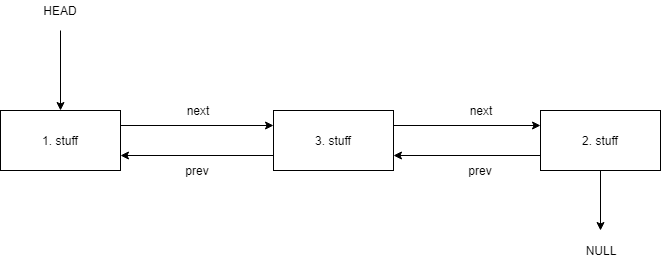
\includegraphics[width=10cm]{proj5_1.png}
 
\end{frame}

\begin{frame}{po řazení}
    
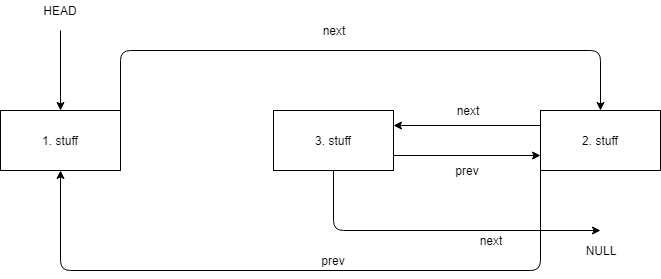
\includegraphics[width=10cm]{proj5_2.png}
    
\end{frame}

\begin{frame}{Děkuji za pozornost}
    
\end{frame}
 
\end{document}